\documentclass[../TDM3_courbe_app.tex]{subfiles}%

\begin{document}
\section[s]"1"{Mouvement hélicoïdal}
\enonce{%
	Un point matériel M a pour équations horaires en coordonnées cylindriques~:
	\[
		\left\{
		\begin{aligned}
			r(t)   & = R    \\
			\th(t) & = \wt  \\
			z(t)   & = \a t
		\end{aligned}
		\right.
		\qavec
		(\a,\w)
		\quad
		\text{des constantes}
	\]
}
\QR{%
	Exprimer le vecteur vitesse et le vecteur accélération dans la base
	cylindrique.
}{%
	On a
	\smallbreak
	\noindent
	\begin{minipage}{0.60\linewidth}
		\begin{align*}
			\OM(t) & = R\ur + \a t\uz                                  \\
			\vf(t) & = \underbracket[1pt]{\cancel{\dot{R}\ur}}_{=0} +
			R\underbracket[1pt]{\tp}_{\mathclap{=\w}}\ut + \a\uz + \a t
			\underbracket[1pt]{\cancel{\dv{\uz}{t}}}_{=0}              \\
			       & = R\w\ut + \a\uz                                  \\
			\af(t) & = R \underbracket[1pt]{\cancel{\dot{\w}}}_{=0}\ut
			-R\w^2\ur + \of                                            \\
			       & = -R\w^2\ur
		\end{align*}
	\end{minipage}
	\hfill
	\begin{minipage}{0.30\linewidth}
		\begin{center}
			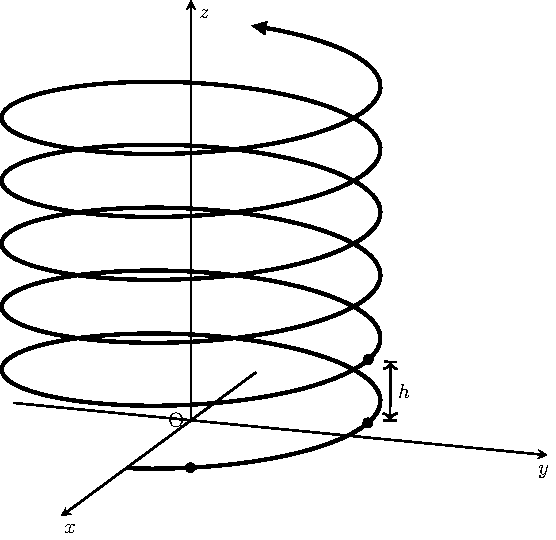
\includegraphics[width=\linewidth]{helix}
		\end{center}
	\end{minipage}
}
\QR{%
	Dessiner l'allure de la trajectoire.
}{%
	Cf.\ ci-dessus.
}
\QR{%
	Déterminer $h$ le pas de l'hélice, c'est-à-dire la distance selon
	l'axe (O$z$) dont sont séparés deux points successifs de la trajectoire
	correspondant à un même angle $\th$ (modulo $2\pi$).
}{%
	Soit $t_0$ un instant quelconque. Un point à ce temps-là est tel que
	\[
		\left\{
		\begin{aligned}
			r(t_0)   & = R      \\
			\th(t_0) & = \wt_0  \\
			z(t_0)   & = \a t_0
		\end{aligned}
		\right.
	\]
	Le premier point qui est au même angle $\th$ mais avec $2\pi$ de plus se
	trouve donc à $t_1$ tel que
	\begin{align*}
		\th(t_1)    & = \th(t_0) + 2\pi
		\\\Lra
		\wt_1       & = \wt_0 + 2\pi
		\\\Lra
		\Aboxed{t_1 & = t_0 + \frac{2\pi}{\w}}
	\end{align*}
	On a alors
	\vspace*{-26pt}
	\begin{gather*}
		z(t_1) - z(t_0) = h = \a t_1 - \a t_0
		\\\Lra
		\boxed{h = 2\pi \frac{\a}{\w}}
	\end{gather*}
}
\QR{%
	Ce mouvement est-il uniforme~? À quelle condition est-il circulaire~?
}{%
	$\norm{\vf} = \sqrt{R^2\w^2+\a^2} = \cte$, donc il est uniforme. Il
	est circulaire ssi \fbox{$\a = 0$}.
}
\QR{%
	Déterminer les coordonnées cartésiennes de ce mouvement.
}{%
	En regardant dans le plan polaire, on trouve $x(t)$ et $y(t)$~:
	\begin{empheq}[box=\fbox, left=\empheqlbrace]{align*}
		x(t) & = R\cos(\wt)\\
		y(t) & = R\sin(\wt)\\
		z(t) & = \a t
	\end{empheq}
}
\end{document}
